
%% bare_conf.tex
%% V1.4b
%% 2015/08/26
%% by Michael Shell
%% See:
%% http://www.michaelshell.org/
%% for current contact information.
%%
%% This is a skeleton file demonstrating the use of IEEEtran.cls
%% (requires IEEEtran.cls version 1.8b or later) with an IEEE
%% conference paper.
%%
%% Support sites:
%% http://www.michaelshell.org/tex/ieeetran/
%% http://www.ctan.org/pkg/ieeetran
%% and
%% http://www.ieee.org/

%%*************************************************************************
%% Legal Notice:
%% This code is offered as-is without any warranty either expressed or
%% implied; without even the implied warranty of MERCHANTABILITY or
%% FITNESS FOR A PARTICULAR PURPOSE! 
%% User assumes all risk.
%% In no event shall the IEEE or any contributor to this code be liable for
%% any damages or losses, including, but not limited to, incidental,
%% consequential, or any other damages, resulting from the use or misuse
%% of any information contained here.
%%
%% All comments are the opinions of their respective authors and are not
%% necessarily endorsed by the IEEE.
%%
%% This work is distributed under the LaTeX Project Public License (LPPL)
%% ( http://www.latex-project.org/ ) version 1.3, and may be freely used,
%% distributed and modified. A copy of the LPPL, version 1.3, is included
%% in the base LaTeX documentation of all distributions of LaTeX released
%% 2003/12/01 or later.
%% Retain all contribution notices and credits.
%% ** Modified files should be clearly indicated as such, including  **
%% ** renaming them and changing author support contact information. **
%%*************************************************************************


% *** Authors should verify (and, if needed, correct) their LaTeX system  ***
% *** with the testflow diagnostic prior to trusting their LaTeX platform ***
% *** with production work. The IEEE's font choices and paper sizes can   ***
% *** trigger bugs that do not appear when using other class files.       ***                          ***
% The testflow support page is at:
% http://www.michaelshell.org/tex/testflow/



\documentclass[conference]{IEEEtran}
\usepackage[utf8]{inputenc}
\usepackage[spanish]{babel}
\usepackage{graphicx}
%\usepackage{subcaption}
%\usepackage[caption=false, font=footnotesize]{subfig}
\usepackage{hyperref}
\usepackage{mathrsfs,amsmath}
\usepackage{array}
\usepackage{mdwmath}
\usepackage{mdwtab}

% Some Computer Society conferences also require the compsoc mode option,
% but others use the standard conference format.
%
% If IEEEtran.cls has not been installed into the LaTeX system files,
% manually specify the path to it like:
% \documentclass[conference]{../sty/IEEEtran}





% Some very useful LaTeX packages include:
% (uncomment the ones you want to load)


% *** MISC UTILITY PACKAGES ***
%
%\usepackage{ifpdf}
% Heiko Oberdiek's ifpdf.sty is very useful if you need conditional
% compilation based on whether the output is pdf or dvi.
% usage:
% \ifpdf
%   % pdf code
% \else
%   % dvi code
% \fi
% The latest version of ifpdf.sty can be obtained from:
% http://www.ctan.org/pkg/ifpdf
% Also, note that IEEEtran.cls V1.7 and later provides a builtin
% \ifCLASSINFOpdf conditional that works the same way.
% When switching from latex to pdflatex and vice-versa, the compiler may
% have to be run twice to clear warning/error messages.






% *** CITATION PACKAGES ***
%
%\usepackage{cite}
% cite.sty was written by Donald Arseneau
% V1.6 and later of IEEEtran pre-defines the format of the cite.sty package
% \cite{} output to follow that of the IEEE. Loading the cite package will
% result in citation numbers being automatically sorted and properly
% "compressed/ranged". e.g., [1], [9], [2], [7], [5], [6] without using
% cite.sty will become [1], [2], [5]--[7], [9] using cite.sty. cite.sty's
% \cite will automatically add leading space, if needed. Use cite.sty's
% noadjust option (cite.sty V3.8 and later) if you want to turn this off
% such as if a citation ever needs to be enclosed in parenthesis.
% cite.sty is already installed on most LaTeX systems. Be sure and use
% version 5.0 (2009-03-20) and later if using hyperref.sty.
% The latest version can be obtained at:
% http://www.ctan.org/pkg/cite
% The documentation is contained in the cite.sty file itself.


\ifCLASSOPTIONcompsoc
    \usepackage[caption=false, font=normalsize, labelfont=sf, textfont=sf]{subfig}
\else
\usepackage[caption=false, font=footnotesize]{subfig}
\fi




% *** GRAPHICS RELATED PACKAGES ***
%
\ifCLASSINFOpdf
  % \usepackage[pdftex]{graphicx}
  % declare the path(s) where your graphic files are
  % \graphicspath{{../pdf/}{../jpeg/}}
  % and their extensions so you won't have to specify these with
  % every instance of \includegraphics
  % \DeclareGraphicsExtensions{.pdf,.jpeg,.png}
\else
  % or other class option (dvipsone, dvipdf, if not using dvips). graphicx
  % will default to the driver specified in the system graphics.cfg if no
  % driver is specified.
  % \usepackage[dvips]{graphicx}
  % declare the path(s) where your graphic files are
  % \graphicspath{{../eps/}}
  % and their extensions so you won't have to specify these with
  % every instance of \includegraphics
  % \DeclareGraphicsExtensions{.eps}
\fi
% graphicx was written by David Carlisle and Sebastian Rahtz. It is
% required if you want graphics, photos, etc. graphicx.sty is already
% installed on most LaTeX systems. The latest version and documentation
% can be obtained at: 
% http://www.ctan.org/pkg/graphicx
% Another good source of documentation is "Using Imported Graphics in
% LaTeX2e" by Keith Reckdahl which can be found at:
% http://www.ctan.org/pkg/epslatex
%
% latex, and pdflatex in dvi mode, support graphics in encapsulated
% postscript (.eps) format. pdflatex in pdf mode supports graphics
% in .pdf, .jpeg, .png and .mps (metapost) formats. Users should ensure
% that all non-photo figures use a vector format (.eps, .pdf, .mps) and
% not a bitmapped formats (.jpeg, .png). The IEEE frowns on bitmapped formats
% which can result in "jaggedy"/blurry rendering of lines and letters as
% well as large increases in file sizes.
%
% You can find documentation about the pdfTeX application at:
% http://www.tug.org/applications/pdftex





% *** MATH PACKAGES ***
%
%\usepackage{amsmath}
% A popular package from the American Mathematical Society that provides
% many useful and powerful commands for dealing with mathematics.
%
% Note that the amsmath package sets \interdisplaylinepenalty to 10000
% thus preventing page breaks from occurring within multiline equations. Use:
%\interdisplaylinepenalty=2500
% after loading amsmath to restore such page breaks as IEEEtran.cls normally
% does. amsmath.sty is already installed on most LaTeX systems. The latest
% version and documentation can be obtained at:
% http://www.ctan.org/pkg/amsmath





% *** SPECIALIZED LIST PACKAGES ***
%
%\usepackage{algorithmic}
% algorithmic.sty was written by Peter Williams and Rogerio Brito.
% This package provides an algorithmic environment fo describing algorithms.
% You can use the algorithmic environment in-text or within a figure
% environment to provide for a floating algorithm. Do NOT use the algorithm
% floating environment provided by algorithm.sty (by the same authors) or
% algorithm2e.sty (by Christophe Fiorio) as the IEEE does not use dedicated
% algorithm float types and packages that provide these will not provide
% correct IEEE style captions. The latest version and documentation of
% algorithmic.sty can be obtained at:
% http://www.ctan.org/pkg/algorithms
% Also of interest may be the (relatively newer and more customizable)
% algorithmicx.sty package by Szasz Janos:
% http://www.ctan.org/pkg/algorithmicx




% *** ALIGNMENT PACKAGES ***
%
%\usepackage{array}
% Frank Mittelbach's and David Carlisle's array.sty patches and improves
% the standard LaTeX2e array and tabular environments to provide better
% appearance and additional user controls. As the default LaTeX2e table
% generation code is lacking to the point of almost being broken with
% respect to the quality of the end results, all users are strongly
% advised to use an enhanced (at the very least that provided by array.sty)
% set of table tools. array.sty is already installed on most systems. The
% latest version and documentation can be obtained at:
% http://www.ctan.org/pkg/array


% IEEEtran contains the IEEEeqnarray family of commands that can be used to
% generate multiline equations as well as matrices, tables, etc., of high
% quality.




% *** SUBFIGURE PACKAGES ***
%\ifCLASSOPTIONcompsoc
%  \usepackage[caption=false,font=normalsize,labelfont=sf,textfont=sf]{subfig}
%\else
%  \usepackage[caption=false,font=footnotesize]{subfig}
%\fi
% subfig.sty, written by Steven Douglas Cochran, is the modern replacement
% for subfigure.sty, the latter of which is no longer maintained and is
% incompatible with some LaTeX packages including fixltx2e. However,
% subfig.sty requires and automatically loads Axel Sommerfeldt's caption.sty
% which will override IEEEtran.cls' handling of captions and this will result
% in non-IEEE style figure/table captions. To prevent this problem, be sure
% and invoke subfig.sty's "caption=false" package option (available since
% subfig.sty version 1.3, 2005/06/28) as this is will preserve IEEEtran.cls
% handling of captions.
% Note that the Computer Society format requires a larger sans serif font
% than the serif footnote size font used in traditional IEEE formatting
% and thus the need to invoke different subfig.sty package options depending
% on whether compsoc mode has been enabled.
%
% The latest version and documentation of subfig.sty can be obtained at:
% http://www.ctan.org/pkg/subfig




% *** FLOAT PACKAGES ***
%
%\usepackage{fixltx2e}
% fixltx2e, the successor to the earlier fix2col.sty, was written by
% Frank Mittelbach and David Carlisle. This package corrects a few problems
% in the LaTeX2e kernel, the most notable of which is that in current
% LaTeX2e releases, the ordering of single and double column floats is not
% guaranteed to be preserved. Thus, an unpatched LaTeX2e can allow a
% single column figure to be placed prior to an earlier double column
% figure.
% Be aware that LaTeX2e kernels dated 2015 and later have fixltx2e.sty's
% corrections already built into the system in which case a warning will
% be issued if an attempt is made to load fixltx2e.sty as it is no longer
% needed.
% The latest version and documentation can be found at:
% http://www.ctan.org/pkg/fixltx2e


%\usepackage{stfloats}
% stfloats.sty was written by Sigitas Tolusis. This package gives LaTeX2e
% the ability to do double column floats at the bottom of the page as well
% as the top. (e.g., "\begin{figure*}[!b]" is not normally possible in
% LaTeX2e). It also provides a command:
%\fnbelowfloat
% to enable the placement of footnotes below bottom floats (the standard
% LaTeX2e kernel puts them above bottom floats). This is an invasive package
% which rewrites many portions of the LaTeX2e float routines. It may not work
% with other packages that modify the LaTeX2e float routines. The latest
% version and documentation can be obtained at:
% http://www.ctan.org/pkg/stfloats
% Do not use the stfloats baselinefloat ability as the IEEE does not allow
% \baselineskip to stretch. Authors submitting work to the IEEE should note
% that the IEEE rarely uses double column equations and that authors should try
% to avoid such use. Do not be tempted to use the cuted.sty or midfloat.sty
% packages (also by Sigitas Tolusis) as the IEEE does not format its papers in
% such ways.
% Do not attempt to use stfloats with fixltx2e as they are incompatible.
% Instead, use Morten Hogholm'a dblfloatfix which combines the features
% of both fixltx2e and stfloats:
%
% \usepackage{dblfloatfix}
% The latest version can be found at:
% http://www.ctan.org/pkg/dblfloatfix




% *** PDF, URL AND HYPERLINK PACKAGES ***
%
%\usepackage{url}
% url.sty was written by Donald Arseneau. It provides better support for
% handling and breaking URLs. url.sty is already installed on most LaTeX
% systems. The latest version and documentation can be obtained at:
% http://www.ctan.org/pkg/url
% Basically, \url{my_url_here}.




% *** Do not adjust lengths that control margins, column widths, etc. ***
% *** Do not use packages that alter fonts (such as pslatex).         ***
% There should be no need to do such things with IEEEtran.cls V1.6 and later.
% (Unless specifically asked to do so by the journal or conference you plan
% to submit to, of course. )


% correct bad hyphenation here
\hyphenation{op-tical net-works semi-conduc-tor}


\begin{document}
%
% paper title
% Titles are generally capitalized except for words such as a, an, and, as,
% at, but, by, for, in, nor, of, on, or, the, to and up, which are usually
% not capitalized unless they are the first or last word of the title.
% Linebreaks \\ can be used within to get better formatting as desired.
% Do not put math or special symbols in the title.
\title{Esteganografía por Enmascaramiento con Eco}


% author names and affiliations
% use a multiple column layout for up to three different
% affiliations
\author{\IEEEauthorblockN{Kaleb Alfaro Badilla}
Email: kaleb.23415@gmail.com}


% conference papers do not typically use \thanks and this command
% is locked out in conference mode. If really needed, such as for
% the acknowledgment of grants, issue a \IEEEoverridecommandlockouts
% after \documentclass

% for over three affiliations, or if they all won't fit within the width
% of the page, use this alternative format:
% 
%\author{\IEEEauthorblockN{Michael Shell\IEEEauthorrefmark{1},
%Homer Simpson\IEEEauthorrefmark{2},
%James Kirk\IEEEauthorrefmark{3}, 
%Montgomery Scott\IEEEauthorrefmark{3} and
%Eldon Tyrell\IEEEauthorrefmark{4}}
%\IEEEauthorblockA{\IEEEauthorrefmark{1}School of Electrical and Computer Engineering\\
%Georgia Institute of Technology,
%Atlanta, Georgia 30332--0250\\ Email: see http://www.michaelshell.org/contact.html}
%\IEEEauthorblockA{\IEEEauthorrefmark{2}Twentieth Century Fox, Springfield, USA\\
%Email: homer@thesimpsons.com}
%\IEEEauthorblockA{\IEEEauthorrefmark{3}Starfleet Academy, San Francisco, California 96678-2391\\
%Telephone: (800) 555--1212, Fax: (888) 555--1212}
%\IEEEauthorblockA{\IEEEauthorrefmark{4}Tyrell Inc., 123 Replicant Street, Los Angeles, California 90210--4321}}




% use for special paper notices
%\IEEEspecialpapernotice{(Invited Paper)}




% make the title area
\maketitle

% As a general rule, do not put math, special symbols or citations
% in the abstract
\begin{abstract}
En este proyecto se pretendió desarrollar una implementación de estenografía por enmascaramiento con eco. Para lograrlo se desarrolló un programa del cual introduce efectos de eco cuyo retardo codifica información. Los datos se recuperan mediante otro programa de decodificación utilizando el método de autocorrelación del Cepstro. Del software desarrollado, se estudió la calidad de la implementación al medir la efectividad de recepción de datos. Finalmente se aplicó la calificación objetiva de calidad de audio perceptiva PEAQ.
\end{abstract}

% no keywords




% For peer review papers, you can put extra information on the cover
% page as needed:
% \ifCLASSOPTIONpeerreview
% \begin{center} \bfseries EDICS Category: 3-BBND \end{center}
% \fi
%
% For peerreview papers, this IEEEtran command inserts a page break and
% creates the second title. It will be ignored for other modes.
\IEEEpeerreviewmaketitle



\section{Introduction}
% no \IEEEPARstart
La esteganografía es una técnica donde la codificación de un mensaje se realiza sobre una señal portadora, de forma tal que pase inadvertido. Sobre las aplicaciones que se encuentra esta técnica, se busca explotar las limitaciones perceptuales humanas para enmascarar los mensajes. El procesamiento digital de señales es utilizada como herramienta para desarrollar aplicaciones esteganográficas en señales audio, imágenes, video y telecomunicaciones. Los sistemas LTI facilitan la implementación y análisis de muchos sistemas esteganográficos. En este proyecto se dio énfasis para implementar un sistema de codificación y decodificación de esteganografía por enmascaramiento con eco para señales de audio.

\section{Sistema general}
La implementación del sistema se encuentra basado con la figura \ref{fig:sistema}. Se encuentran dos programas importantes: el codificador y el decodificador. El primero es aquel que realiza la incorporación de datos utilizando retardos de la señal audio. Los retardos se encuentran modulados de acuerdo a los bits relacionados con los metadatos. El codificador cuando soluciona, entrega un archivo de audio codificado, este es introducido al decodificador para recuperar la información. El decodificador genera un archivo de metadatos en función de los datos que recupere del archivo de audio.

\begin{figure}[h]
\centering
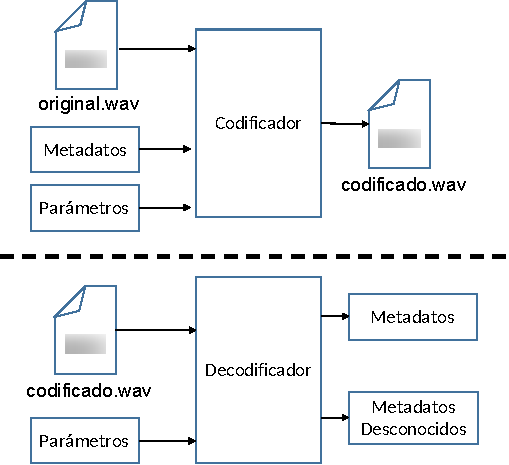
\includegraphics[scale=0.7]{sistema.pdf}
\caption{Diagrama del sistema implementado. Al codificaodr se le introducen los parámetros de codificación, los metadatos para codificar y la canción en formato WAV. El decodificador toma el archivo de audio generado del codificador y toma los parámetros para recuperar los metadatos.}
\label{fig:sistema}
\end{figure}

\subsection{Codificador}
El método de codificación consistió de manejar dos sistemas LTI para generar ecos. Uno relacionado con la codificación del $0$ lógico \eqref{eq:k0} y otro para el $1$ lógico \eqref{eq:k1}. El procedimiento para enmascarar los datos consiste en dividir el vector de audio en una cantidad finita de ventanas; a cada una se le aplica la multiplicación punto a punto con la ventana de Blackman \eqref{eq:bm}. De esta forma se generan $x_N(n)$ ventanas; a cada una de ellas se le realiza una convolución discreta con $h_0(n)$ o $h_1(n)$ generando un $y_N(n)$ ventanas resultantes. Para combinar estas ventanas y reconstruir el archivo de audio original se realiza la técnica de solapamiento y suma, tal como se muestra en la figura \ref{fig:solapadd}.
\begin{equation}
H_0(z)=1+\alpha_0 z^{-t_0}
\label{eq:k0}
\end{equation}
\begin{equation}
H_1(z)=1+\alpha_1 z^{-t_1}
\label{eq:k1}
\end{equation}

\begin{equation}
v(n)=0.42 - 0.5 \cos \left(  \frac{2\pi n}{N-1}\right) + 0.08 \cos \left(  \frac{4\pi n}{N-1}\right)
\label{eq:bm}
\end{equation}

\begin{figure}[h]
\centering
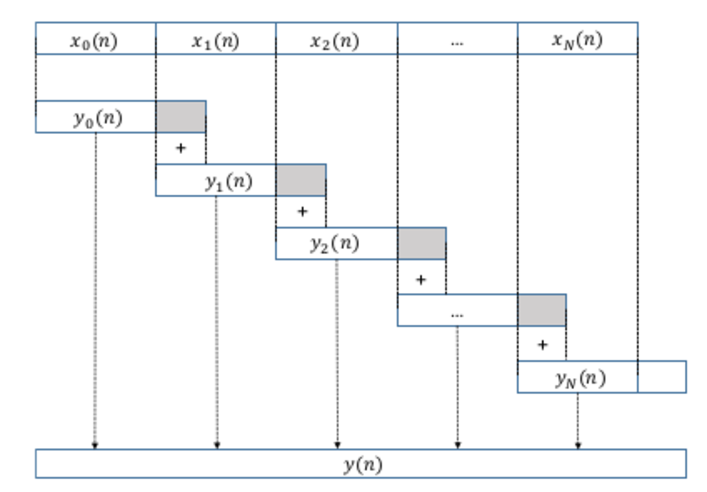
\includegraphics[scale=0.6]{solapadd.pdf}
\caption{Método de solapamiento y suma para reconstruir una señal después de enventanar la señal original y realizarle una convolución discreta.}
\label{fig:solapadd}
\end{figure}

\subsection{Decodificador}
De acuerdo a la bibliografía \cite{IEEEhowto:datahiding2}, se decidió utilizar el método de autocorrelación del Cepstro \eqref{eq:rcc}. Este consiste en ventanar el archivo de audio codificado, multiplicar punto a punto cada ventana por la ventana de Blackman \eqref{eq:bm}, realizar el cálculo de la autocorrelación del Cepstro a cada uno e identificar el bit registrado por el codificador. La secuencia de bits se puede recuperar utilizando la ecuación \eqref{eq:bit}, esta ecuación es aplicada para el k-ésima ventana $x_k(n)$. Con base a la secuencia de bits $B(k)$, se realiza escritura del archivo original.

\begin{equation}
R_{cc_k}(n) = \mathscr{F}^{-1} \left \{  [ln( \mathscr{F} \left \{ x_k(n) \right \} )]^2 \right \}
\label{eq:rcc}
\end{equation}

\begin{equation}
B(k) = \begin{cases}
1 &\text{si $|R_{cc,k}(t_1)|>|R_{cc}(t_0)|$}\\
0 &\text{si $|R_{cc,k}(t_1)|<|R_{cc}(t_0)|$}
\end{cases}
\label{eq:bit}
\end{equation}

\section{Resultados}
\subsection{Autocorrelación del Cepstro}
Para visualizar la codificación de los ecos sobre las ventanas se presentan las figuras \ref{fig:rcc1} y \ref{fig:rcc0}. En ellas se reciben los bits enviados mediante la codificación por eco.

\begin{figure}
\centering
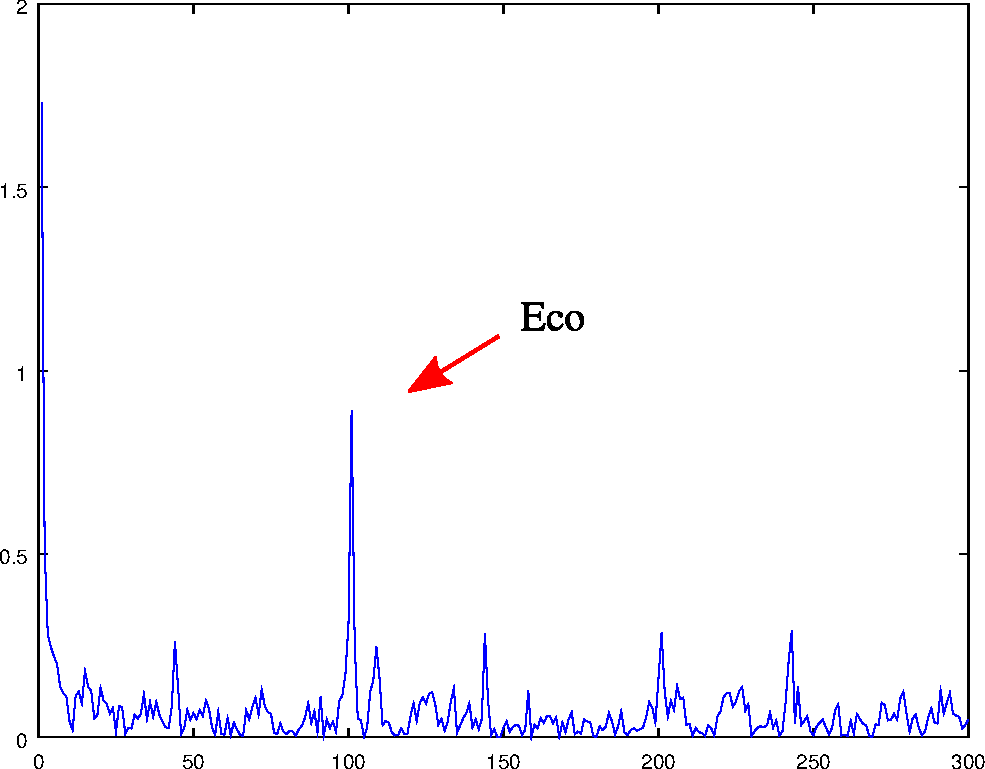
\includegraphics[scale=0.4]{rcc.pdf}
\caption{Visualización de la autocorrelación del Cepstro cuando se encuentra un eco decodificado como un 1 lógico sobre la muestra $t_1=100$.}
\label{fig:rcc1}
\end{figure}

\begin{figure}
\centering
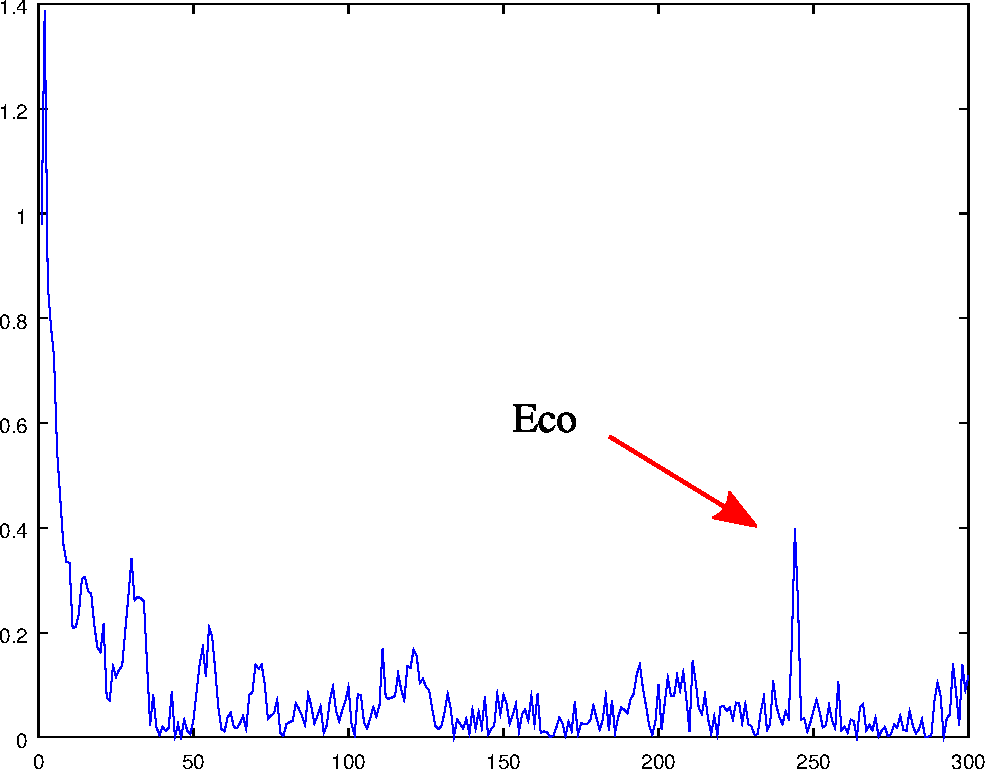
\includegraphics[scale=0.4]{rcc_0.pdf}
\caption{Visualización de la autocorrelación del Cepstro cuando se encuentra un eco decodificado como un 1 lógico sobre la muestra $t_0=243$.}
\label{fig:rcc0}
\end{figure}

\subsection{Análisis de error de bit de llegada}

Se realizó una secuencia de pruebas del sistema completo variando los parámetros de codificación. De esta forma para encontrar el comportamiento en la llegada congruente de los bits recibidos por el decodificador de acuerdo a una referencia. De los resultados obtenidos se presentan las figuras \ref{fig:1000}, \ref{fig:5000}, \ref{fig:10000} y \ref{fig:15000}. En ellas se realizaron las mismas pruebas sobre tres canciones diferentes de 2 minutos cada una. Se realizó variaciones sobre el tamaño de la ventana, el largo del retardo y la atenuación del eco. El retardo del cero se fija $3/2$ veces mayor que del uno. Asumiendo que un sistema aleatorio se esperaría que la llegada de datos tenga un porcentaje de error de 50\%, se observa que existe un umbral donde en conjunto el retardo y la amplitud del eco empieza a ser legible su decodificación. Esto se considera porque los porcentajes de error empiezan a bajar a 8-20\%. Se observan tendencias como al incrementar el valor de la atenuación, mejora la recepción de dato. Asimismo para el retardo fijado para la codificación. Existe una variabilidad en los porcentajes de error de las canciones, pero se suele seguir la misma tendencia entre ellas. Se observa también que al incrementar el tamaño de la ventana comienza a mejorar la recepción correcta de datos; aunque esto reduce drásticamente el ancho de banda para enviar datos por segundo.

\begin{figure}[h]
    \centering
  \subfloat[]{%
        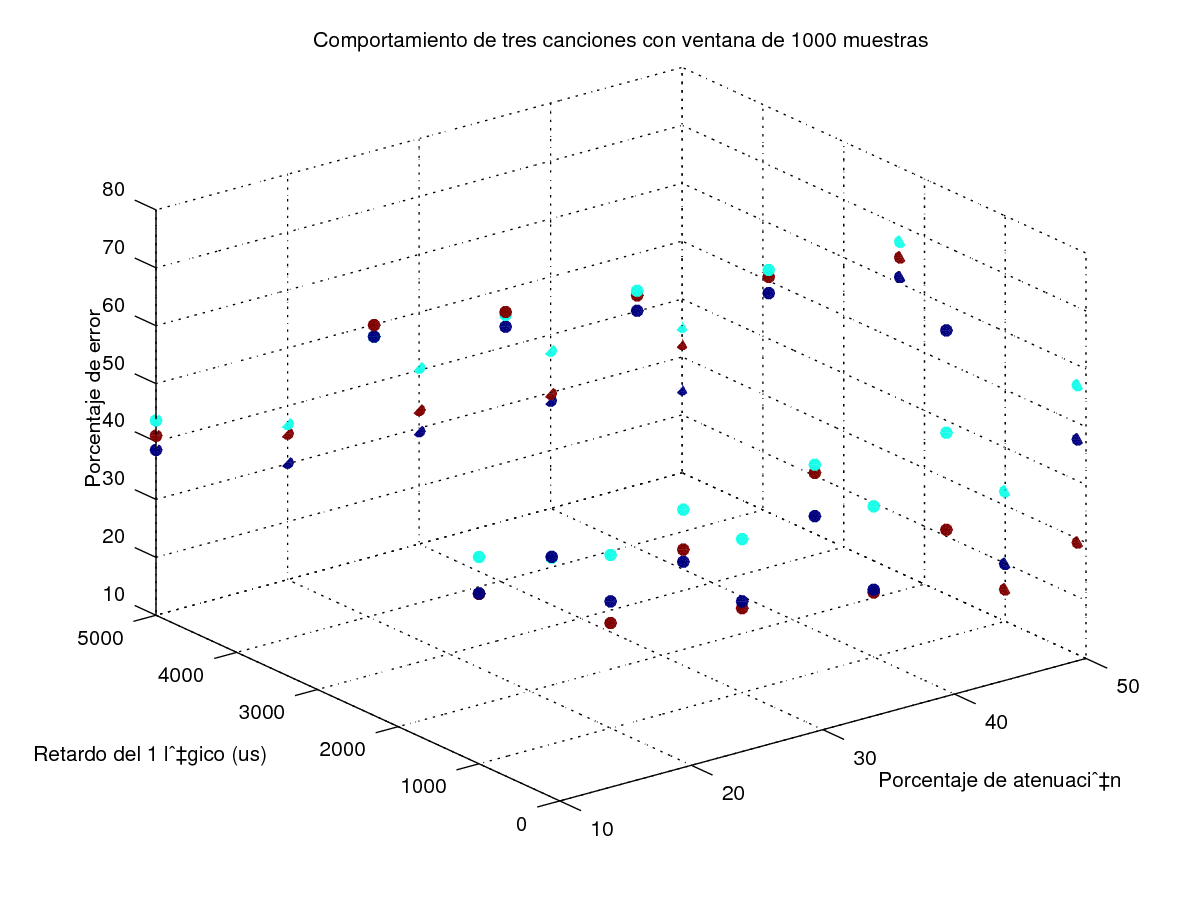
\includegraphics[width=0.9\linewidth]{1000-1.png}}
\\
  \subfloat[]{%
        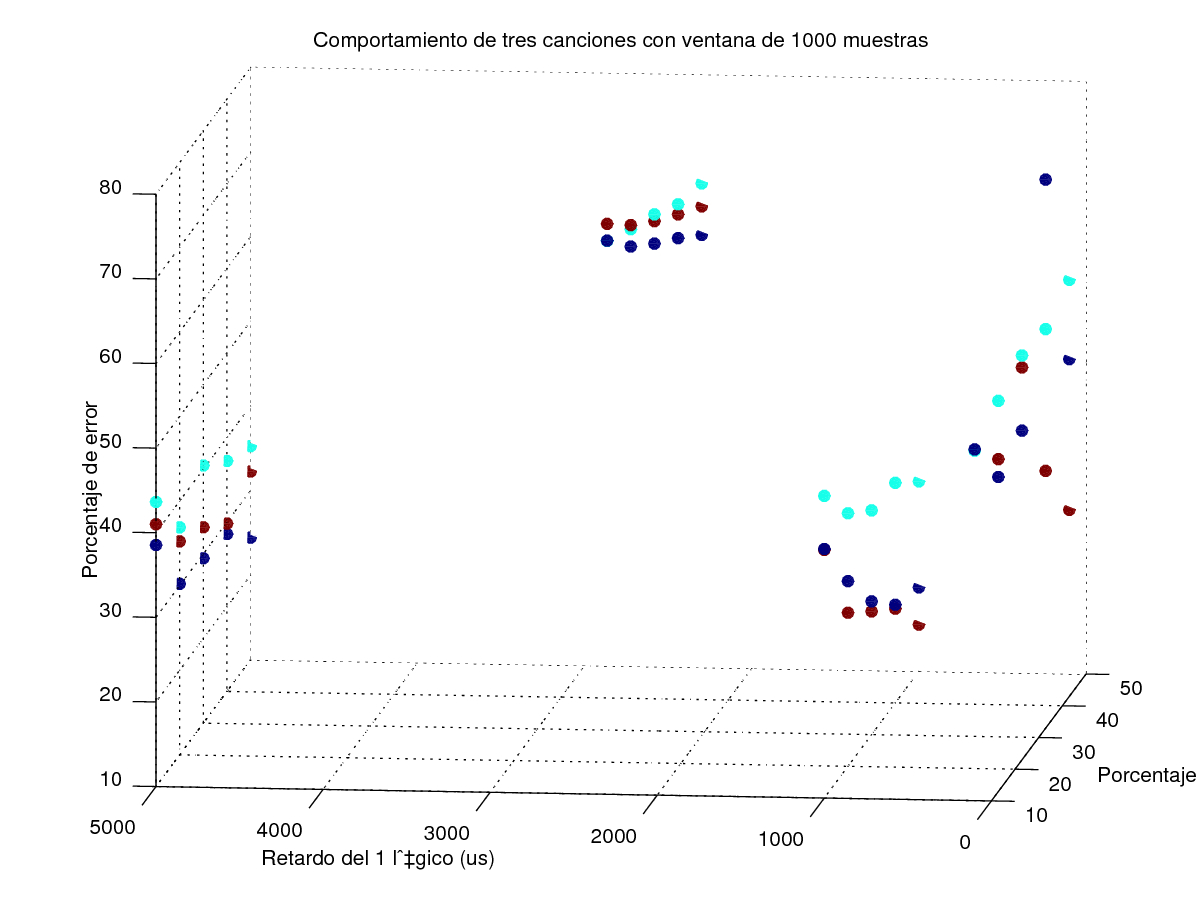
\includegraphics[width=0.9\linewidth]{1000-2.png}}

  \caption{Porcentaje de error de llegada de bits en función de la atenuación y el retardo del eco. El tamaño de la ventana se fijo en 1000 muestras. Cada color representa una canción distinta. $BW=44.1bps$ para $Fs=44.1$kHz.}
  \label{fig:1000} 
\end{figure}

\begin{figure}[h]
    \centering
  \subfloat[]{%
        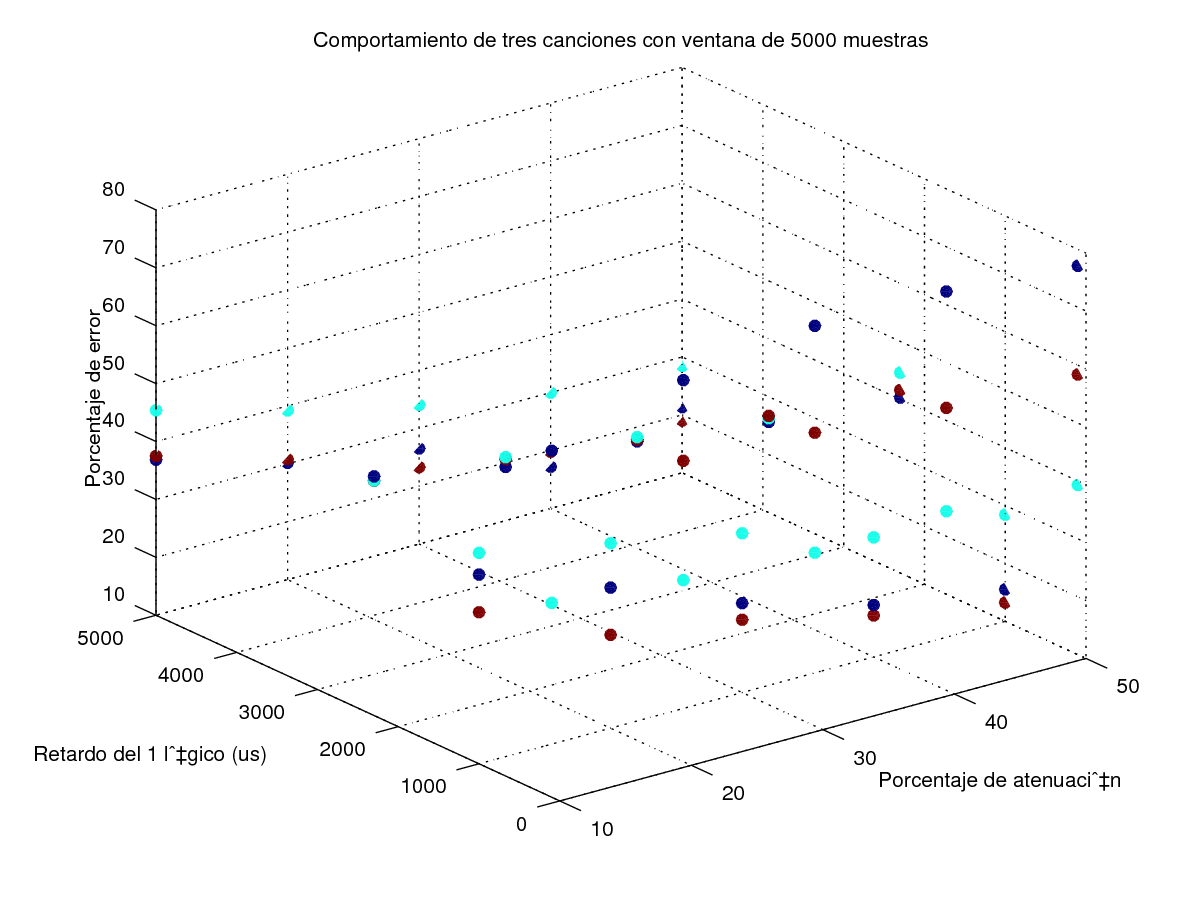
\includegraphics[width=0.9\linewidth]{5000-1.png}}
\\
  \subfloat[]{%
        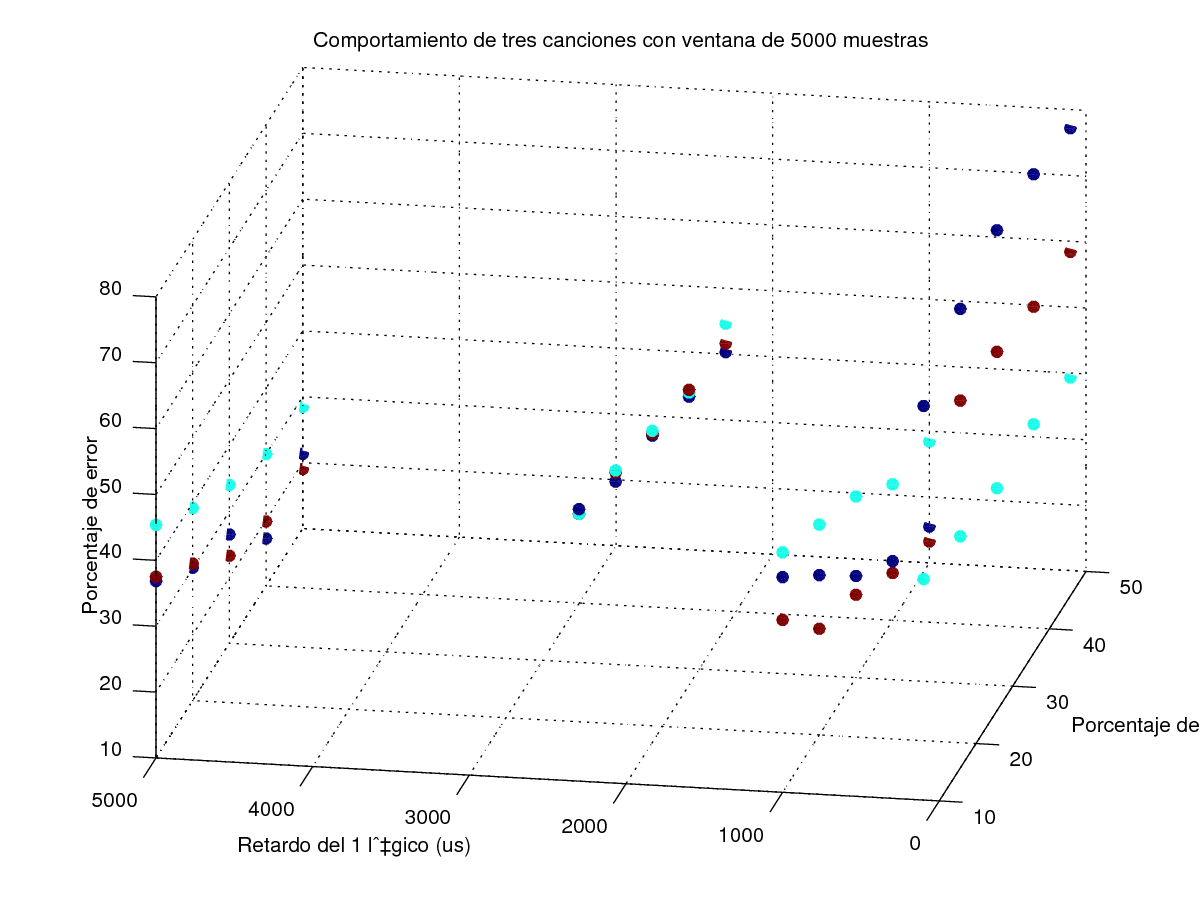
\includegraphics[width=0.9\linewidth]{5000-2.png}}

  \caption{Porcentaje de error de llegada de bits en función de la atenuación y el retardo del eco. El tamaño de la ventana se fijo en 5000 muestras. Cada color representa una canción distinta. $BW=8.82bps$ para $Fs=44.1$kHz.}
  \label{fig:5000} 
\end{figure}

\begin{figure}[h]
    \centering
  \subfloat[]{%
        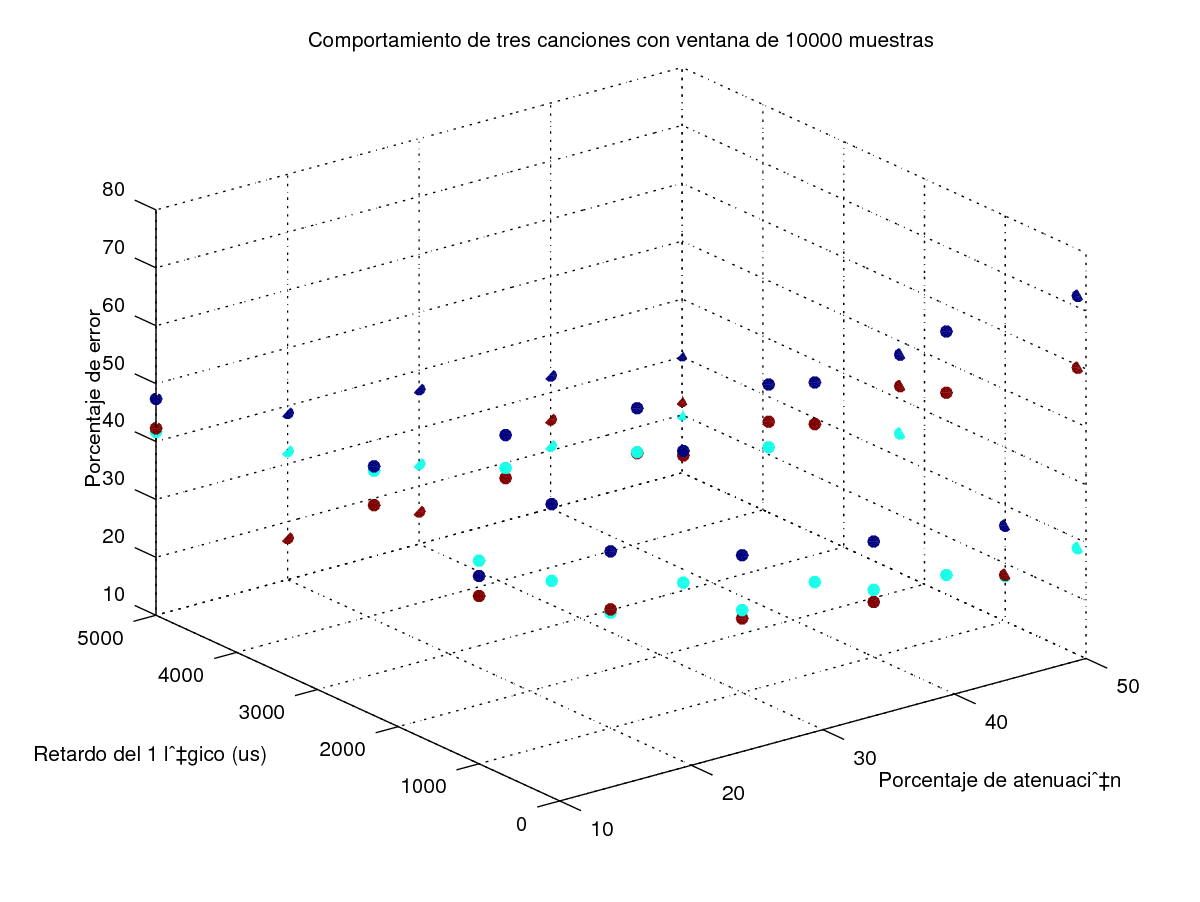
\includegraphics[width=0.9\linewidth]{10000-1.png}}
\\
  \subfloat[]{%
        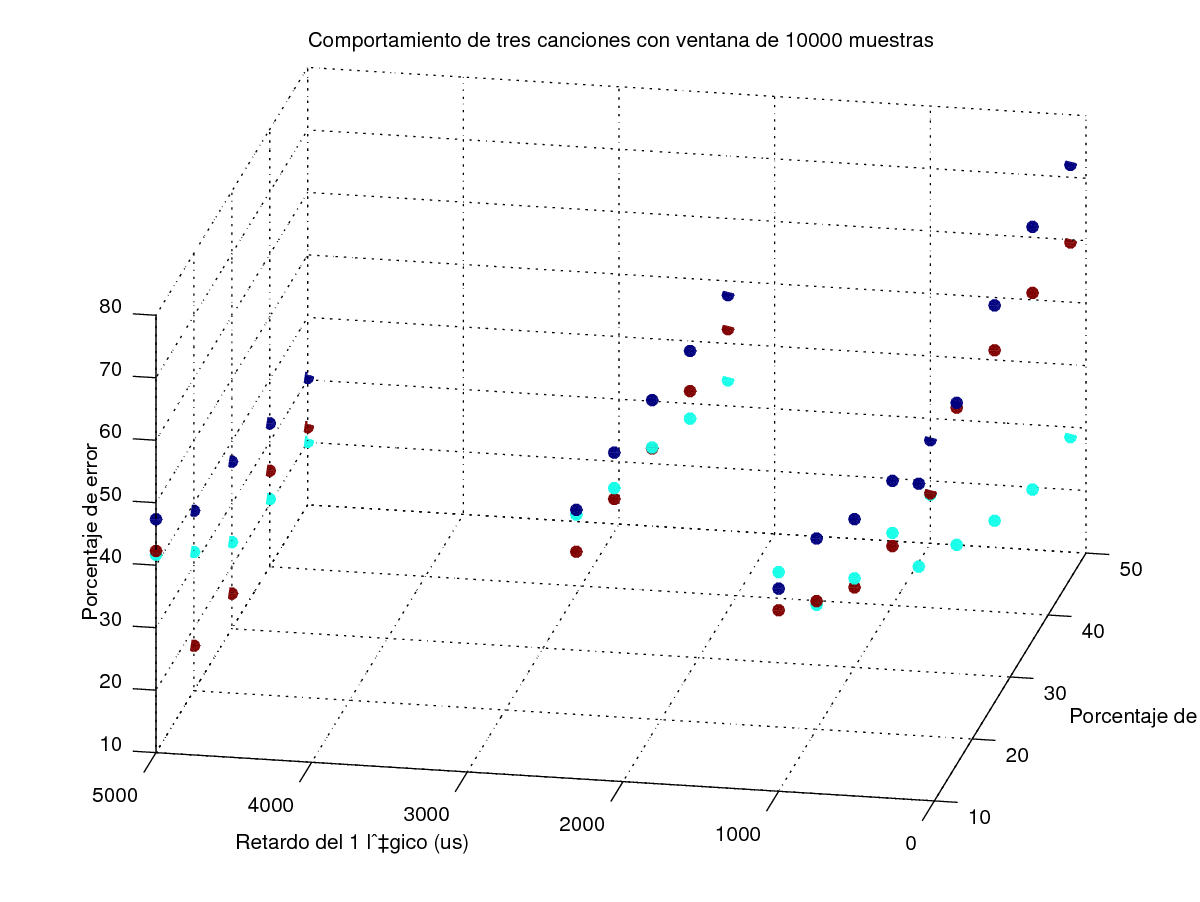
\includegraphics[width=0.9\linewidth]{10000-2.png}}
 
  \caption{Porcentaje de error de llegada de bits en función de la atenuación y el retardo del eco. El tamaño de la ventana se fijo en 10000 muestras. Cada color representa una canción distinta. $BW=4.41bps$ para $Fs=44.1$kHz.}
  \label{fig:10000} 
\end{figure}

\begin{figure}[h]
    \centering
  \subfloat[]{%
        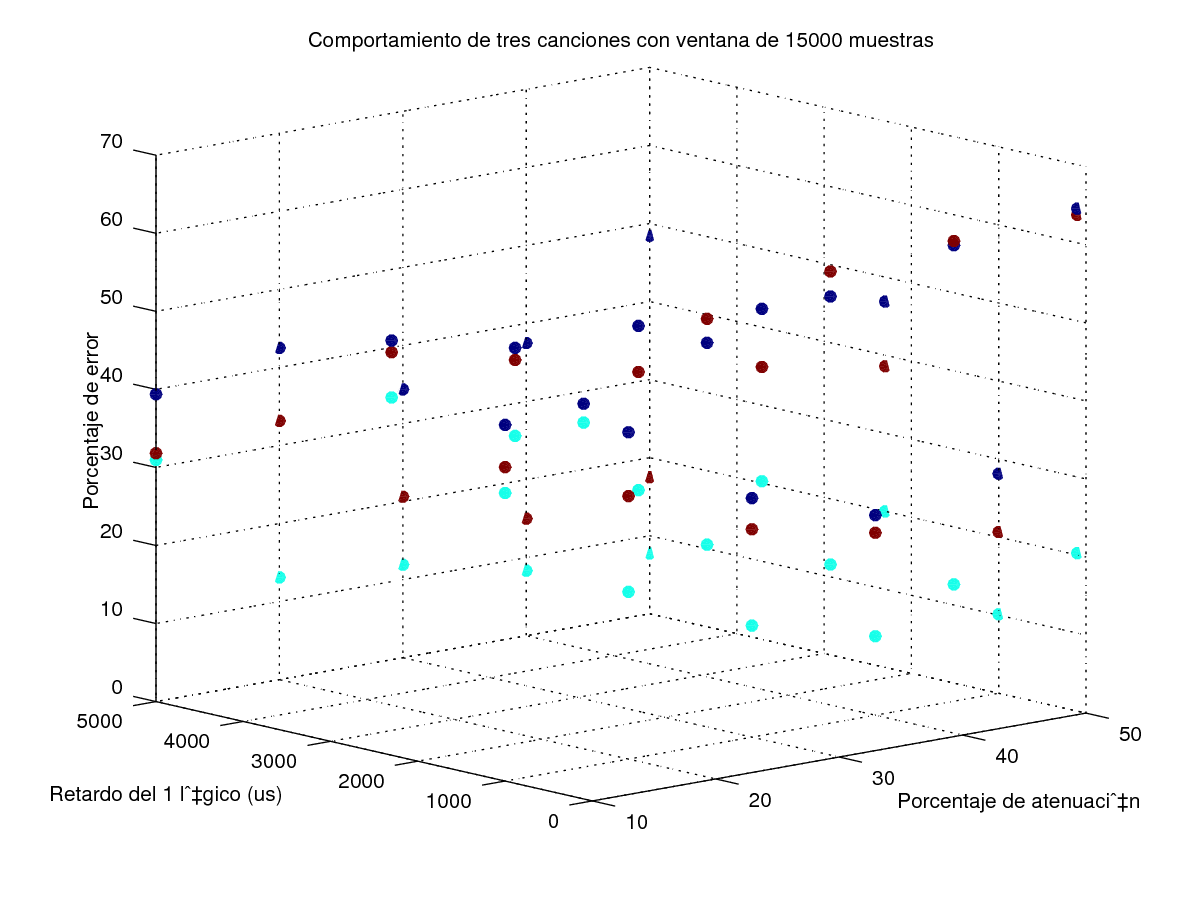
\includegraphics[width=0.9\linewidth]{15000-2.png}}
\\
  \subfloat[]{%
        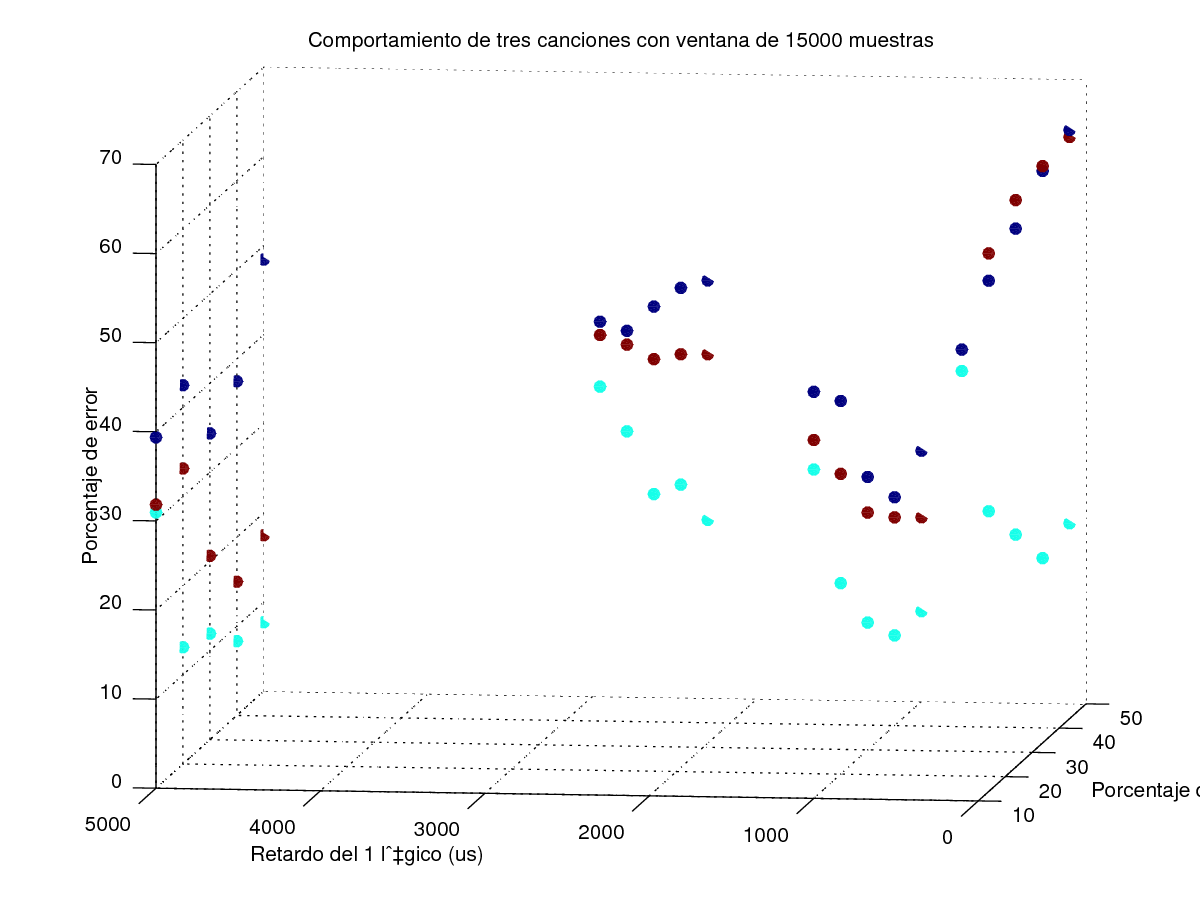
\includegraphics[width=0.9\linewidth]{15000-1.png}}
 
  \caption{Porcentaje de error de llegada de bits en función de la atenuación y el retardo del eco. El tamaño de la ventana se fijo en 15000 muestras. Cada color representa una canción distinta. $BW=2.94$ para $Fs=44.1$kHz.}
  \label{fig:15000} 
\end{figure}

\subsection{Relación con la calificación ODG del PEAQ}
Bajo la premisa que si al mejorar porcentaje de error en la recepción de datos, se empeora la calificación perceptiva del audio original, se realizó graficar dicha relación. El PEAQ utilizado se recuperó de la referencia \cite{PEAQ}  En la figura \ref{fig:odg} se observa dicha gráfica. De acuerdo con ella, no se observa una tendencia clara para justificar que la llegada de datos de forma confiable viole la calidad de audio. Asimismo, la calificación en general se encuentra muy mala en general para todas las muestras realizadas. Se explica porque el método utilizado para codificar, vuelve el audio de estereo a mono, afectando gravemente la calificación.

\begin{figure}[h]
\centering
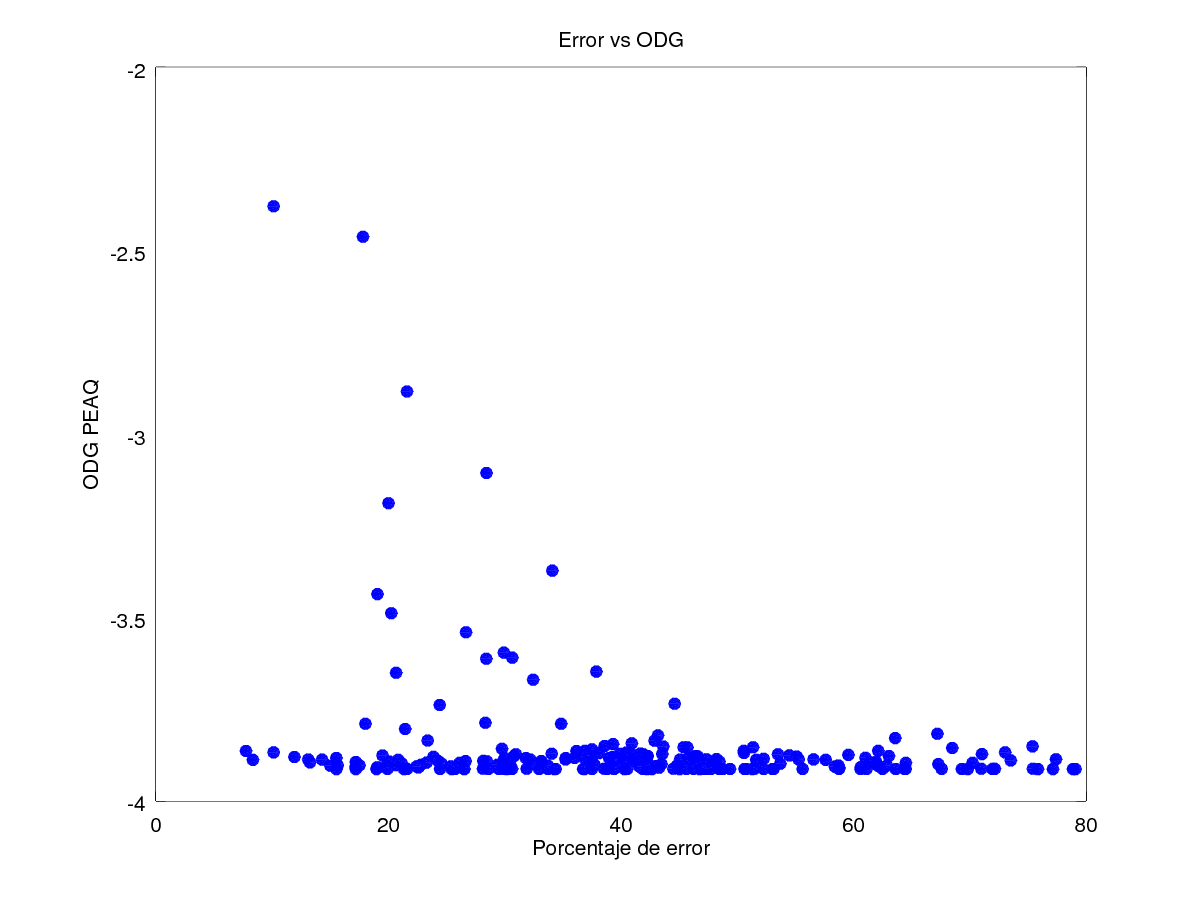
\includegraphics[scale=0.5]{errvsodg.png}
\caption{Relación del porcentaje de error y del grado de calificación objetiva de percepción de calidad de audio.}
\label{fig:odg}
\end{figure}
% You must have at least 2 lines in the paragraph with the drop letter
% (should never be an issue)

\section{Conclusiones}
\begin{enumerate}
\item Existe una relación entre la recepción congruente de los datos en función del largo del retardo y la atenuación del eco.
\item Hay una variabilidad en el porcentaje de error de los datos por canción, pero se mantienen tendencias.
\item Al incrementar el tamaño de la ventana, se mejora el porcentaje de error, pero empeora el ancho de banda.
\item No se encontró una relación clara sobre la calificación ODG del PEAQ y el porcentaje de error de recepción de datos en esta implementación.
\end{enumerate}

\section{Recomendaciones}
\begin{enumerate}
\item Aprovechar los archivos de audio estéreo para incrementar el ancho de banda efectivo por dos canales.
\item Probar con diferentes ventanas para comprobar si se puede recuperar los datos de una manera más efectiva.

\end{enumerate}
% An example of a floating figure using the graphicx package.
% Note that \label must occur AFTER (or within) \caption.
% For figures, \caption should occur after the \includegraphics.
% Note that IEEEtran v1.7 and later has special internal code that
% is designed to preserve the operation of \label within \caption
% even when the captionsoff option is in effect. However, because
% of issues like this, it may be the safest practice to put all your
% \label just after \caption rather than within \caption{}.
%
% Reminder: the "draftcls" or "draftclsnofoot", not "draft", class
% option should be used if it is desired that the figures are to be
% displayed while in draft mode.
%
%\begin{figure}[!t]
%\centering
%\includegraphics[width=2.5in]{myfigure}
% where an .eps filename suffix will be assumed under latex, 
% and a .pdf suffix will be assumed for pdflatex; or what has been declared
% via \DeclareGraphicsExtensions.
%\caption{Simulation results for the network.}
%\label{fig_sim}
%\end{figure}

% Note that the IEEE typically puts floats only at the top, even when this
% results in a large percentage of a column being occupied by floats.


% An example of a double column floating figure using two subfigures.
% (The subfig.sty package must be loaded for this to work.)
% The subfigure \label commands are set within each subfloat command,
% and the \label for the overall figure must come after \caption.
% \hfil is used as a separator to get equal spacing.
% Watch out that the combined width of all the subfigures on a 
% line do not exceed the text width or a line break will occur.
%
%\begin{figure*}[!t]
%\centering
%\subfloat[Case I]{\includegraphics[width=2.5in]{box}%
%\label{fig_first_case}}
%\hfil
%\subfloat[Case II]{\includegraphics[width=2.5in]{box}%
%\label{fig_second_case}}
%\caption{Simulation results for the network.}
%\label{fig_sim}
%\end{figure*}
%
% Note that often IEEE papers with subfigures do not employ subfigure
% captions (using the optional argument to \subfloat[]), but instead will
% reference/describe all of them (a), (b), etc., within the main caption.
% Be aware that for subfig.sty to generate the (a), (b), etc., subfigure
% labels, the optional argument to \subfloat must be present. If a
% subcaption is not desired, just leave its contents blank,
% e.g., \subfloat[].


% An example of a floating table. Note that, for IEEE style tables, the
% \caption command should come BEFORE the table and, given that table
% captions serve much like titles, are usually capitalized except for words
% such as a, an, and, as, at, but, by, for, in, nor, of, on, or, the, to
% and up, which are usually not capitalized unless they are the first or
% last word of the caption. Table text will default to \footnotesize as
% the IEEE normally uses this smaller font for tables.
% The \label must come after \caption as always.
%
%\begin{table}[!t]
%% increase table row spacing, adjust to taste
%\renewcommand{\arraystretch}{1.3}
% if using array.sty, it might be a good idea to tweak the value of
% \extrarowheight as needed to properly center the text within the cells
%\caption{An Example of a Table}
%\label{table_example}
%\centering
%% Some packages, such as MDW tools, offer better commands for making tables
%% than the plain LaTeX2e tabular which is used here.
%\begin{tabular}{|c||c|}
%\hline
%One & Two\\
%\hline
%Three & Four\\
%\hline
%\end{tabular}
%\end{table}


% Note that the IEEE does not put floats in the very first column
% - or typically anywhere on the first page for that matter. Also,
% in-text middle ("here") positioning is typically not used, but it
% is allowed and encouraged for Computer Society conferences (but
% not Computer Society journals). Most IEEE journals/conferences use
% top floats exclusively. 
% Note that, LaTeX2e, unlike IEEE journals/conferences, places
% footnotes above bottom floats. This can be corrected via the
% \fnbelowfloat command of the stfloats package.


% conference papers do not normally have an appendix




% trigger a \newpage just before the given reference
% number - used to balance the columns on the last page
% adjust value as needed - may need to be readjusted if
% the document is modified later
%\IEEEtriggeratref{8}
% The "triggered" command can be changed if desired:
%\IEEEtriggercmd{\enlargethispage{-5in}}

% references section

% can use a bibliography generated by BibTeX as a .bbl file
% BibTeX documentation can be easily obtained at:
% http://mirror.ctan.org/biblio/bibtex/contrib/doc/
% The IEEEtran BibTeX style support page is at:
% http://www.michaelshell.org/tex/ieeetran/bibtex/
%\bibliographystyle{IEEEtran}
% argument is your BibTeX string definitions and bibliography database(s)
%\bibliography{IEEEabrv,../bib/paper}
%
% <OR> manually copy in the resultant .bbl file
% set second argument of \begin to the number of references
% (used to reserve space for the reference number labels box)
\begin{thebibliography}{1}


\bibitem{IEEEhowto:datahiding}
T.~Kim P.~Dutta, D.~Bhattacharyya. Data hiding in audio signal: a review. \hskip 1em plus
 0.5em minus 0.4em\relax  \emph{International Journal of Database Theory and Application}, 2, 2009. Available from: \url{http://www.sersc.org/journals/IJDTA/vol2_no2/1.pdf}

\bibitem{IEEEhowto:datahiding2}
S. Behal N. Kaur. Audio steganography techniques - a survey. \emph{International Journal of
Engineering Research and Applications}, 4:94–100, 2014. Available from: \url{http://www.ijera.
com/papers/Vol4_issue6/Version\%205/P0460594100.pdf}.

\bibitem{IEEEhowto:datahiding3}
V. Korzhik. Audio watermarking based on echo hiding with zero error probability. 
\emph{International Journal of Computer Science and Applications}, 10:1–10, 2013. Available from:
\url{http://www.tmrfindia.org/ijcsa/v10i11.pdf}.

\bibitem{PEAQ}
Repositorio \url{https://github.com/akinori-ito/peaqb-fast}.
\end{thebibliography}




% that's all folks
\end{document}


